% ============================================================
%  DISCOVERY CURRICULUM — Journey 3, Module 1
%  "Vectors and Linear Maps"
%  Compile with: pdflatex J3_M1.tex  (run twice for references)
% ============================================================

\documentclass[12pt, a4paper]{article}

\usepackage[a4paper, top=2.5cm, bottom=2.5cm, left=2.8cm, right=2.8cm, headheight=15pt]{geometry}
\usepackage{amsmath, amssymb, amsthm}
\usepackage{xcolor}
\usepackage{mdframed}
\usepackage{enumitem}
\usepackage{tikz}
\usetikzlibrary{arrows.meta, positioning, calc}
\usepackage{pgfplots}
\pgfplotsset{compat=1.18}
\usepackage{booktabs}
\usepackage{fancyhdr}
\usepackage{titlesec}
\usepackage{parskip}
\usepackage{hyperref}
\hypersetup{colorlinks=true, linkcolor=NavyBlue, urlcolor=NavyBlue}

% ── Colours ─────────────────────────────────────────────────
\definecolor{NavyBlue}{HTML}{1A3A5C}
\definecolor{MidBlue}{HTML}{2E6DA4}
\definecolor{Gold}{HTML}{C8922A}
\definecolor{LightBlue}{HTML}{EBF2FA}
\definecolor{LightGold}{HTML}{FDF4E3}
\definecolor{DarkGrey}{HTML}{3A3A3A}
\definecolor{BoxGreen}{HTML}{E8F5E9}
\definecolor{SidebarGrey}{HTML}{F5F5F5}

% ── Section formatting ───────────────────────────────────────
\titleformat{\section}{\Large\bfseries\color{NavyBlue}}{}{0em}{}[{\color{MidBlue}\vspace{2pt}\rule{\linewidth}{1.5pt}}]
\titleformat{\subsection}{\large\bfseries\color{MidBlue}}{}{0em}{}

% ── Header / Footer ─────────────────────────────────────────
\pagestyle{fancy}
\fancyhf{}
\fancyhead[L]{\small\color{DarkGrey}\textit{Discovery Curriculum}}
\fancyhead[R]{\small\color{DarkGrey}\textit{Journey 3 $\cdot$ Module 1}}
\fancyfoot[C]{\small\color{MidBlue}\thepage}
\renewcommand{\headrulewidth}{0.4pt}

% ── Environments ─────────────────────────────────────────────
\newmdenv[
  backgroundcolor=NavyBlue!7,
  linecolor=NavyBlue, linewidth=2pt,
  leftline=true, rightline=false, topline=false, bottomline=false,
  innerleftmargin=14pt, innerrightmargin=10pt,
  innertopmargin=10pt, innerbottommargin=10pt,
  skipabove=14pt, skipbelow=10pt
]{puzzlebox}

\newmdenv[
  backgroundcolor=LightGold,
  linecolor=Gold, linewidth=2pt,
  leftline=true, rightline=false, topline=false, bottomline=false,
  innerleftmargin=14pt, innerrightmargin=10pt,
  innertopmargin=10pt, innerbottommargin=10pt,
  skipabove=14pt, skipbelow=10pt
]{discoverybox}

\newmdenv[
  backgroundcolor=LightBlue,
  linecolor=MidBlue, linewidth=1.5pt,
  roundcorner=4pt,
  innerleftmargin=14pt, innerrightmargin=10pt,
  innertopmargin=10pt, innerbottommargin=10pt,
  skipabove=14pt, skipbelow=10pt
]{namebox}

\newmdenv[
  backgroundcolor=BoxGreen,
  linecolor=DarkGrey!35, linewidth=1pt,
  roundcorner=4pt,
  innerleftmargin=14pt, innerrightmargin=10pt,
  innertopmargin=10pt, innerbottommargin=10pt,
  skipabove=14pt, skipbelow=10pt
]{reflectionbox}

\newmdenv[
  backgroundcolor=SidebarGrey,
  linecolor=Gold, linewidth=1.2pt,
  leftline=true, rightline=false, topline=false, bottomline=false,
  innerleftmargin=12pt, innerrightmargin=10pt,
  innertopmargin=7pt, innerbottommargin=7pt,
  skipabove=10pt, skipbelow=10pt
]{thought}

\newcounter{problem}
\newenvironment{problem}[1][]{%
  \refstepcounter{problem}%
  \par\vspace{6pt}%
  \noindent\textbf{\color{MidBlue}Problem \theproblem}%
  \ifx&#1&\else\ \textit{(#1)}\fi\textbf{.}\enskip
}{\par\vspace{4pt}}

\newcounter{deepproblem}
\newenvironment{deepproblem}[1][]{%
  \refstepcounter{deepproblem}%
  \par\vspace{6pt}%
  \noindent\textbf{\color{NavyBlue}$\bigstar$\ Deep Problem \thedeepproblem}%
  \ifx&#1&\else\ \textit{(#1)}\fi\textbf{.}\enskip
}{\par\vspace{4pt}}

% ============================================================
\begin{document}
% ============================================================

\thispagestyle{empty}
\begin{center}
{\small\color{MidBlue}\textbf{DISCOVERY CURRICULUM}\quad$\cdot$\quad\textbf{JOURNEY 3: LINEAR STRUCTURE}}

\vspace{0.6cm}
{\color{NavyBlue}\rule{\linewidth}{2pt}}
\vspace{0.5cm}

{\Huge\bfseries\color{NavyBlue}Module 1}\\[0.3cm]
{\LARGE\bfseries\color{MidBlue}Vectors and Linear Maps}\\[0.4cm]
{\color{Gold}\rule{0.4\linewidth}{1.2pt}}\\[0.4cm]
{\large\itshape\color{DarkGrey}
A vector is not an arrow. An arrow is one picture\\[0.15cm]
of something much more general.}

\vspace{1cm}
\begin{tabular}{rl}
\color{DarkGrey}\textbf{Journey}           & Journey 3 --- Linear Structure \\[4pt]
\color{DarkGrey}\textbf{Module}            & 1 of 6 \\[4pt]
\color{DarkGrey}\textbf{Prerequisites}     & Journey 1 (functions, graphs); Journey 2 (gradient, Jacobian) \\[4pt]
\color{DarkGrey}\textbf{You will discover} & Vector spaces, linear maps, kernel, image, dimension \\[4pt]
\color{DarkGrey}\textbf{Format}            & 8 problems $+$ 3 deep problems $\approx$ 13 pages \\
\end{tabular}

\vspace{1cm}
{\color{NavyBlue}\rule{\linewidth}{2pt}}
\end{center}

\vspace{0.5cm}

\noindent\textbf{Opening Journey 3.}
In Journey~2 you met the gradient $\nabla f$ --- a vector. The Jacobian $Df$ --- a matrix. The Hessian $H$ --- also a matrix. These appeared naturally as tools for understanding change. But what exactly is a vector? What is a matrix? And why do they behave the way they do?

\medskip
Journey~3 builds the answer from scratch. Linear algebra is the mathematics of \emph{linear structure}: spaces where addition and scaling are defined, and maps between them that respect those operations. It is the most widely used branch of mathematics in science and engineering, and it underlies --- in ways you will see explicitly --- everything from differential equations to quantum mechanics to Google's search algorithm.

\newpage

% ============================================================
\section{Part 1 \texorpdfstring{---}{--} The Puzzle}
% ============================================================

\begin{puzzlebox}
\textbf{The Opening Puzzle.}

Here are five very different mathematical objects:
\begin{enumerate}[noitemsep, label=(\roman*)]
  \item Arrows in the plane $\mathbb{R}^2$
  \item Polynomials $p(x) = a_0 + a_1 x + a_2 x^2$ of degree $\leq 2$
  \item Continuous functions $f : [0,1] \to \mathbb{R}$
  \item Solutions to the ODE $y'' + y = 0$
  \item $2 \times 2$ matrices
\end{enumerate}

\textbf{Question 1.} For each: can you add two objects of the same type and get another object of the same type? Can you multiply by a real number and stay in the type?

\textbf{Question 2.} Do these operations --- addition and scalar multiplication --- behave the same way across all five types? Write down three properties they all share.

\textbf{Question 3.} These five things are all examples of the same abstract structure. What should we call it?
\end{puzzlebox}

\medskip
The puzzle reveals that the essential structure of a ``vector'' is not the arrow picture --- that is just one example. The essential structure is the algebraic behaviour: addition and scalar multiplication satisfying certain rules. Once you recognise this, you can do linear algebra on polynomials, functions, differential equations, and matrices --- not just arrows.

% ============================================================
\section{Part 2 \texorpdfstring{---}{--} Exploration}
% ============================================================

\subsection{Step 1: The axioms}

\begin{problem}
\label{prob:vs_axioms}
A \textbf{vector space} over $\mathbb{R}$ is a set $V$ with two operations --- addition $+: V \times V \to V$ and scalar multiplication $\cdot : \mathbb{R} \times V \to V$ --- satisfying eight axioms.

\begin{enumerate}[label=(\alph*), topsep=2pt]
  \item Write down what you think the eight axioms should be, based on how addition and multiplication by numbers works for ordinary arrows. Do not look them up --- derive them from what you know.
  \item Verify all eight axioms for the set of polynomials of degree $\leq n$, with the natural addition and scalar multiplication.
  \item Verify them for the set of solutions to $y'' + y = 0$. (From Module 5, Journey 2, the general solution is $A\cos x + B\sin x$.) How many ``free'' numbers does a solution require?
  \item Show that the set $\{(x, y) \in \mathbb{R}^2 : x + y = 1\}$ is \emph{not} a vector space. Which axiom fails?
  \item Show that the set $\{(x, y) \in \mathbb{R}^2 : x + y = 0\}$ \emph{is} a vector space. What is the zero vector?
\end{enumerate}
\end{problem}

\begin{thought}
\textbf{Why axioms?}
When you write down the axioms for a vector space, you are doing something subtle: you are distilling the \emph{minimum requirements} for a structure to behave like vectors. Any theorem you can prove from these axioms alone will hold simultaneously for arrows, polynomials, functions, matrices, and anything else satisfying the axioms. This is the power of abstraction --- you prove a theorem once and it applies everywhere. The danger of abstraction is losing contact with examples. The discipline of linear algebra is to move fluently between the abstract axioms and the concrete instances, neither forgetting the examples nor being trapped by any single one.
\end{thought}

\subsection{Step 2: Subspaces, span, and linear independence}

\begin{problem}
\label{prob:subspace}
A \textbf{subspace} of $V$ is a non-empty subset $W \subseteq V$ that is closed under addition and scalar multiplication (equivalently: $\alpha \mathbf{u} + \beta \mathbf{v} \in W$ whenever $\mathbf{u}, \mathbf{v} \in W$ and $\alpha, \beta \in \mathbb{R}$).

\begin{enumerate}[label=(\alph*), topsep=2pt]
  \item Which of the following are subspaces of $\mathbb{R}^3$?
    \begin{itemize}[noitemsep]
      \item The $xy$-plane: $\{(x,y,0)\}$
      \item The line $\{(t, 2t, 3t) : t \in \mathbb{R}\}$
      \item The set $\{(x,y,z) : x^2 + y^2 + z^2 = 1\}$ (the unit sphere)
      \item The set $\{(x,y,z) : x + 2y - z = 0\}$
    \end{itemize}
  \item The \textbf{span} of vectors $\mathbf{v}_1, \ldots, \mathbf{v}_k$ is all linear combinations $\alpha_1\mathbf{v}_1 + \cdots + \alpha_k\mathbf{v}_k$. Describe the span of $(1,0,0)$ and $(0,1,0)$ geometrically.
  \item Vectors $\mathbf{v}_1, \ldots, \mathbf{v}_k$ are \textbf{linearly independent} if the only solution to $\alpha_1\mathbf{v}_1 + \cdots + \alpha_k\mathbf{v}_k = \mathbf{0}$ is $\alpha_1 = \cdots = \alpha_k = 0$. Test independence for: $\{(1,2,3),\, (2,4,6)\}$; $\{(1,0,0),\, (0,1,0),\, (0,0,1)\}$; $\{1, x, x^2\}$ as polynomials.
  \item Explain in one sentence why a linearly dependent set is ``redundant.''
  \item The polynomials $1, x, x^2, \ldots, x^n$ span the space of polynomials of degree $\leq n$. Are they linearly independent?
\end{enumerate}
\end{problem}

\subsection{Step 3: Basis and dimension}

\begin{problem}
\label{prob:basis_dim}
A \textbf{basis} of $V$ is a set of vectors that is both linearly independent and spans $V$.
\begin{enumerate}[label=(\alph*), topsep=2pt]
  \item Find two different bases of $\mathbb{R}^2$. Do they have the same number of vectors?
  \item Find a basis for the subspace $\{(x,y,z) : x + 2y - z = 0\} \subseteq \mathbb{R}^3$.
  \item The space of polynomials of degree $\leq 2$ has basis $\{1, x, x^2\}$. Find a different basis for the same space.
  \item \textbf{Key theorem (accept without proof for now):} Any two bases of $V$ have the same number of elements. This number is the \textbf{dimension} of $V$.
  What is the dimension of $\mathbb{R}^n$? Of polynomials of degree $\leq n$? Of $2\times 2$ matrices? Of solutions to $y''+y=0$?
  \item The space of \emph{all} continuous functions on $[0,1]$ is infinite-dimensional. Why? What does an infinite basis look like?
\end{enumerate}
\end{problem}

\begin{center}
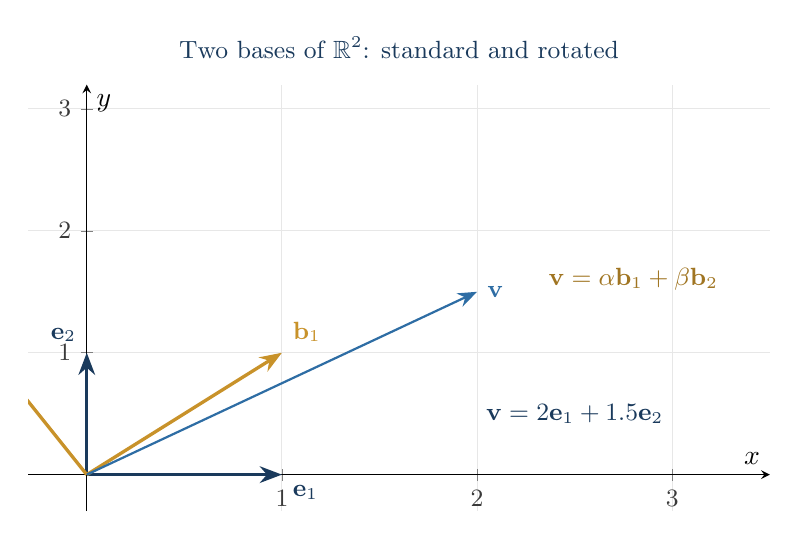
\begin{tikzpicture}
\begin{axis}[
  width=11cm, height=7cm,
  axis lines=center,
  xlabel={$x$}, ylabel={$y$},
  xmin=-0.3, xmax=3.5, ymin=-0.3, ymax=3.2,
  xtick={1,2,3}, ytick={1,2,3},
  tick label style={font=\small, color=DarkGrey},
  grid=major, grid style={DarkGrey!12},
  title={\small\color{NavyBlue}Two bases of $\mathbb{R}^2$: standard and rotated},
]
% Standard basis vectors
\draw[-{Stealth[length=8pt]}, NavyBlue, very thick] (axis cs:0,0) -- (axis cs:1,0) node[below right, font=\small] {$\mathbf{e}_1$};
\draw[-{Stealth[length=8pt]}, NavyBlue, very thick] (axis cs:0,0) -- (axis cs:0,1) node[above left, font=\small] {$\mathbf{e}_2$};
% Alternative basis
\draw[-{Stealth[length=8pt]}, Gold, very thick] (axis cs:0,0) -- (axis cs:1,1) node[above right, font=\small] {$\mathbf{b}_1$};
\draw[-{Stealth[length=8pt]}, Gold, very thick] (axis cs:0,0) -- (axis cs:-0.5,1) node[above left, font=\small] {$\mathbf{b}_2$};
% A vector expressed in both
\draw[-{Stealth[length=7pt]}, MidBlue, thick] (axis cs:0,0) -- (axis cs:2,1.5) node[right, font=\small] {$\mathbf{v}$};
\node[font=\small, color=NavyBlue] at (axis cs:2.5, 0.5) {$\mathbf{v} = 2\mathbf{e}_1 + 1.5\mathbf{e}_2$};
\node[font=\small, color=Gold!80!black] at (axis cs:2.8, 1.6) {$\mathbf{v} = \alpha\mathbf{b}_1 + \beta\mathbf{b}_2$};
\end{axis}
\end{tikzpicture}
\end{center}

\subsection{Step 4: Linear maps}

\begin{problem}
\label{prob:linear_map}
A \textbf{linear map} (linear transformation) $T : V \to W$ satisfies:
\[
  T(\mathbf{u} + \mathbf{v}) = T(\mathbf{u}) + T(\mathbf{v}) \quad \text{and} \quad T(\alpha \mathbf{v}) = \alpha T(\mathbf{v})
\]
for all $\mathbf{u},\mathbf{v} \in V$ and $\alpha \in \mathbb{R}$.

\begin{enumerate}[label=(\alph*), topsep=2pt]
  \item Which of the following are linear maps from $\mathbb{R}^2$ to $\mathbb{R}^2$?
    \begin{itemize}[noitemsep]
      \item $T(x,y) = (2x, 3y)$
      \item $T(x,y) = (x+1, y)$
      \item $T(x,y) = (x+y, x-y)$
      \item $T(x,y) = (x^2, y)$
    \end{itemize}
  \item Differentiation $D : p(x) \mapsto p'(x)$ is a linear map on polynomials. Verify both linearity conditions.
  \item Integration $I : f \mapsto \int_0^x f(t)\,dt$ is a linear map on continuous functions. Verify.
  \item The evaluation map $\text{ev}_a : f \mapsto f(a)$ is a linear map from functions to $\mathbb{R}$. Verify.
  \item A linear map is completely determined by what it does to a basis. If $T(\mathbf{e}_1) = (1,2)$ and $T(\mathbf{e}_2) = (3,4)$, find $T(2\mathbf{e}_1 - \mathbf{e}_2)$ and $T(5, -3)$.
\end{enumerate}
\end{problem}

\begin{thought}
\textbf{Linearity is everywhere.}
Differentiation is linear ($\frac{d}{dx}(f+g) = f'+g'$, $\frac{d}{dx}(cf) = cf'$). Integration is linear ($\int(f+g) = \int f + \int g$). The Fourier transform is linear. The Laplace transform is linear. The expectation of a random variable is linear. The operation of matrix multiplication is linear. Quantum mechanical operators are linear. The linearity of these operations is not an accident --- it is the mathematical signature of \emph{superposition}, the principle that causes, effects, inputs, and outputs can be decomposed and recombined. Wherever superposition holds in physics, a linear map underlies it.
\end{thought}

\subsection{Step 5: Kernel and image}

\begin{problem}
\label{prob:ker_im}
For a linear map $T : V \to W$, define:
\[
  \ker T = \{\mathbf{v} \in V : T(\mathbf{v}) = \mathbf{0}\}, \qquad
  \text{im}\, T = \{T(\mathbf{v}) : \mathbf{v} \in V\}.
\]
\begin{enumerate}[label=(\alph*), topsep=2pt]
  \item Prove that $\ker T$ is a subspace of $V$ and $\text{im}\, T$ is a subspace of $W$.
  \item For $T : \mathbb{R}^3 \to \mathbb{R}^2$ given by $T(x,y,z) = (x+y, y+z)$: find $\ker T$ and $\text{im}\, T$. What are their dimensions?
  \item For the differentiation map $D : \text{Poly}_{\leq 3} \to \text{Poly}_{\leq 2}$: what is $\ker D$? What is $\text{im}\, D$?
  \item $T$ is \textbf{injective} (one-to-one) if and only if $\ker T = \{\mathbf{0}\}$. $T$ is \textbf{surjective} (onto) if and only if $\text{im}\, T = W$. Test your maps from (b) and (c) for each.
  \item \textbf{Rank-Nullity Theorem}: $\dim(\ker T) + \dim(\text{im}\, T) = \dim V$. Verify this for (b) and (c). Why must this be true?
\end{enumerate}
\end{problem}

\begin{problem}
\label{prob:coordinates}
Once a basis $\mathcal{B} = \{\mathbf{b}_1, \ldots, \mathbf{b}_n\}$ is chosen, every vector $\mathbf{v} \in V$ has a unique coordinate representation $[\mathbf{v}]_\mathcal{B} = (\alpha_1, \ldots, \alpha_n)$ where $\mathbf{v} = \sum \alpha_i \mathbf{b}_i$.
\begin{enumerate}[label=(\alph*), topsep=2pt]
  \item In $\mathbb{R}^2$, find the coordinates of $\mathbf{v} = (5, 3)$ with respect to the basis $\mathbf{b}_1 = (1,1)$, $\mathbf{b}_2 = (1,-1)$.
  \item The polynomial $p(x) = 3 - 2x + x^2$ has coordinates $(3,-2,1)$ with respect to the standard basis $\{1, x, x^2\}$. Find its coordinates with respect to $\{1, x-1, (x-1)^2\}$.
  \item The differentiation map $D$ on $\text{Poly}_{\leq 2}$ sends $\{1, x, x^2\} \to \{0, 1, 2x\}$. Write the coordinates of $D(1), D(x), D(x^2)$ in terms of the standard basis. Arrange them as columns of a matrix. You have just computed the \textbf{matrix of a linear map}.
  \item Verify that this matrix, applied to the coordinate vector of $p(x) = 3 - 2x + x^2$, gives the coordinate vector of $p'(x)$.
  \item What is the kernel of this matrix? Compare with the kernel of the differentiation map.
\end{enumerate}
\end{problem}

% ============================================================
\section{Part 3 \texorpdfstring{---}{--} Discovery}
% ============================================================

\begin{discoverybox}
\textbf{What have we built?}

\textbf{First.} A vector space is any set with addition and scalar multiplication satisfying eight axioms. Examples: $\mathbb{R}^n$, polynomials, continuous functions, solutions to linear ODEs, matrices.

\textbf{Second.} Subspace, span, linear independence, basis, dimension are the structural vocabulary. Every finite-dimensional space looks like $\mathbb{R}^n$ once a basis is chosen --- but the choice of basis is an additional structure, not intrinsic.

\textbf{Third.} Linear maps are the natural structure-preserving maps between vector spaces. They are determined by their action on a basis. Kernel and image measure ``what gets destroyed'' and ``what gets produced.''

\textbf{Fourth.} The matrix of a linear map is what you get when you choose bases and write everything in coordinates. The abstract linear map is basis-independent; the matrix depends on the choice of basis.

\medskip
\textbf{The key insight.} Once a basis is fixed, a linear map becomes a matrix. Linear algebra in coordinates (matrices, columns, rows) is the same subject as linear algebra abstractly (maps, kernels, images) --- but the abstract version reveals structure that coordinates can obscure. The art of linear algebra is knowing when to use each perspective.
\end{discoverybox}

% ============================================================
\section{Part 4 \texorpdfstring{---}{--} Naming the Ideas}
% ============================================================

\begin{namebox}
\textbf{Vector space.}

A \textbf{vector space} over $\mathbb{R}$ is a set $V$ with operations $+$ and $\cdot$ satisfying: commutativity and associativity of $+$; existence of $\mathbf{0}$ and negatives; distributivity of $\cdot$ over both $+$ operations; $1\cdot\mathbf{v} = \mathbf{v}$.

A \textbf{subspace} is a non-empty subset closed under $+$ and $\cdot$.

A \textbf{basis} is a linearly independent spanning set. The \textbf{dimension} $\dim V$ is the (well-defined) size of any basis.
\end{namebox}

\begin{namebox}
\textbf{Linear maps and the Rank-Nullity Theorem.}

$T: V \to W$ is \textbf{linear} if $T(\alpha\mathbf{u} + \beta\mathbf{v}) = \alpha T(\mathbf{u}) + \beta T(\mathbf{v})$ for all $\mathbf{u},\mathbf{v},\alpha,\beta$.

$\ker T$ (nullspace) and $\text{im}\,T$ (column space) are subspaces.

\textbf{Rank-Nullity Theorem:} $\dim(\ker T) + \dim(\text{im}\,T) = \dim V$.

$T$ is injective $\iff$ $\ker T = \{0\}$. $T$ is surjective $\iff$ $\text{im}\,T = W$. $T$ is an isomorphism (bijective linear map) $\iff$ $\dim V = \dim W$ and $T$ is injective.

Every $n$-dimensional vector space is isomorphic to $\mathbb{R}^n$.
\end{namebox}

% ============================================================
\section{Part 5 \texorpdfstring{---}{--} Deep Problems}
% ============================================================

\begin{deepproblem}[Infinite-dimensional spaces]
\begin{enumerate}[label=(\alph*)]
  \item The space $C[0,1]$ of continuous functions on $[0,1]$ is infinite-dimensional. Exhibit an infinite linearly independent set.
  \item The space $\ell^2$ of square-summable sequences $(a_1, a_2, a_3, \ldots)$ with $\sum a_n^2 < \infty$ is a vector space. Verify closure under addition: if $\sum a_n^2 < \infty$ and $\sum b_n^2 < \infty$, does $\sum (a_n + b_n)^2 < \infty$? (Use the Cauchy-Schwarz inequality.)
  \item In $\ell^2$, the standard basis vectors $\mathbf{e}_k = (0,\ldots,0,1,0,\ldots)$ (1 in position $k$) form an orthonormal set. Does every element of $\ell^2$ have a unique expansion in this basis? What does this mean for convergence?
  \item The space $L^2[0,1]$ of square-integrable functions (with $\int_0^1 f^2 < \infty$) is the function-space analogue of $\ell^2$. The functions $\{1, \cos 2\pi nx, \sin 2\pi nx : n \geq 1\}$ form an orthonormal basis. This is the Fourier basis. Each function has a unique expansion --- its Fourier series. Does this remind you of anything from Module 5, Journey 2?
\end{enumerate}
\end{deepproblem}

\begin{deepproblem}[Quotient spaces and the first isomorphism theorem]
\begin{enumerate}[label=(\alph*)]
  \item Let $W \subseteq V$ be a subspace. Define the \textbf{quotient space} $V/W$ as the set of cosets $\mathbf{v} + W = \{\mathbf{v} + \mathbf{w} : \mathbf{w} \in W\}$. Define addition and scalar multiplication on cosets and verify $V/W$ is a vector space.
  \item Compute $\dim(V/W)$ when $\dim V = 5$ and $\dim W = 2$.
  \item For a linear map $T : V \to W$, define $\tilde{T} : V/\ker T \to \text{im}\,T$ by $\tilde{T}(\mathbf{v} + \ker T) = T(\mathbf{v})$. Show $\tilde{T}$ is well-defined, linear, and an isomorphism. This is the \textbf{first isomorphism theorem} for vector spaces: $V/\ker T \cong \text{im}\,T$.
  \item Deduce the Rank-Nullity theorem from the first isomorphism theorem.
  \item The first isomorphism theorem is also true for groups, rings, and modules --- in fact, for any algebraic structure with a suitable notion of quotient. What does this suggest about the relationship between vector spaces and other algebraic structures? (This is Journey 7's territory.)
\end{enumerate}
\end{deepproblem}

\begin{deepproblem}[Dual spaces]
The \textbf{dual space} $V^*$ of a vector space $V$ is the set of all linear maps from $V$ to $\mathbb{R}$ (called \textbf{linear functionals}).
\begin{enumerate}[label=(\alph*)]
  \item Show $V^*$ is itself a vector space under pointwise addition and scalar multiplication.
  \item For $V = \mathbb{R}^n$, show that every linear functional has the form $f(\mathbf{x}) = \mathbf{a}\cdot\mathbf{x}$ for some fixed $\mathbf{a} \in \mathbb{R}^n$. Hence $V^* \cong V$.
  \item For $V = C[0,1]$, integration $f \mapsto \int_0^1 f(x)\,dx$ is a linear functional. Evaluation $\text{ev}_a : f \mapsto f(a)$ is another. Are these in $V^*$?
  \item Given a basis $\{\mathbf{b}_1, \ldots, \mathbf{b}_n\}$ of $V$, define the \textbf{dual basis} $\{\mathbf{b}^1, \ldots, \mathbf{b}^n\}$ of $V^*$ by $\mathbf{b}^i(\mathbf{b}_j) = \delta_{ij}$ (Kronecker delta). Show the dual basis is a basis for $V^*$.
  \item In physics, the distinction between a vector and its dual --- between $\mathbf{v} \in V$ and $\phi \in V^*$ --- is the distinction between contravariant and covariant tensors. In general relativity, spacetime geometry requires both. Write one sentence explaining why the gradient $\nabla f$ is naturally an element of $V^*$ rather than $V$.
\end{enumerate}
\end{deepproblem}

% ============================================================
\section{Part 6 \texorpdfstring{---}{--} Reflection}
% ============================================================

\begin{reflectionbox}
\textbf{Your reflection task.}

\begin{enumerate}
  \item \textbf{On abstraction.} You now have a definition of ``vector'' that includes arrows, polynomials, functions, and solutions to differential equations. Does this feel like it clarifies what a vector is, or does it feel like it obscures the original geometric intuition? Write two paragraphs arguing opposite positions.

  \item \textbf{On the matrix of a linear map.} The matrix of a linear map depends on the choice of basis. The linear map itself does not. This means a single abstract map can be represented by infinitely many different matrices. What does this say about the relationship between a mathematical object and its representation? Can you think of analogies in other domains?

  \item \textbf{On the Rank-Nullity Theorem.} The theorem says: whatever dimensions the kernel and image have, they add up to $\dim V$. In plain language: a linear map can ``destroy'' some dimensions (the kernel) and ``produce'' others (the image), but the total count is conserved. Does this feel like a conservation law? Is it?

  \item \textbf{Looking ahead.} Module~2 studies matrices as representations of linear maps: how to compute with them, what their rows and columns mean, and how to solve systems of linear equations. You have already seen the matrix of the differentiation map. What do you expect the matrix of the integration map to look like?
\end{enumerate}
\end{reflectionbox}

\medskip
\noindent\textbf{Looking ahead.}
Module~2 takes the abstract theory of Module~1 and asks: how do you compute? Given a linear map as a matrix, how do you find its kernel (solve a linear system), its image (column space), and whether it is invertible? The techniques --- row reduction, Gaussian elimination, determinants --- are the computational heart of linear algebra, and they connect back to the systems of equations you have been solving throughout Journey~2.

\vspace{1.4cm}
\begin{center}
{\color{MidBlue}\rule{0.5\linewidth}{0.8pt}}\\[6pt]
{\small\color{DarkGrey}\textit{End of Journey 3, Module 1 --- Vectors and Linear Maps}}\\[4pt]
{\small\color{DarkGrey}Continue to: \textbf{Module 2 --- Matrices and Systems}}\\[6pt]
{\color{MidBlue}\rule{0.5\linewidth}{0.8pt}}
\end{center}

\end{document}